\begin{figure}[!hb]
    \centering
    a)
    \begin{minipage}{.45\textwidth}
        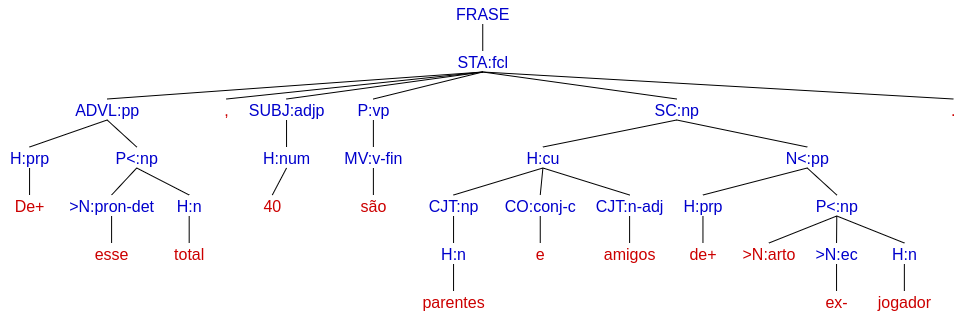
\includegraphics[width=\linewidth]{imagens/ec_bosque_ec_tree_orig.png}
        \caption{árvore original}
    % \end{subfigure}
    \end{minipage}
    % 
    b)
    \begin{minipage}{.45\textwidth}
        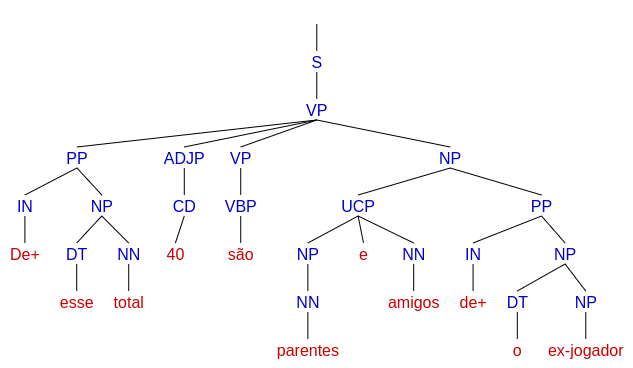
\includegraphics[width=\linewidth]{imagens/ec_bosque_ec_tree_trans.png}
        \caption{árvore transduzida}
    \end{minipage}
    c)
    \begin{minipage}{.45\textwidth}
        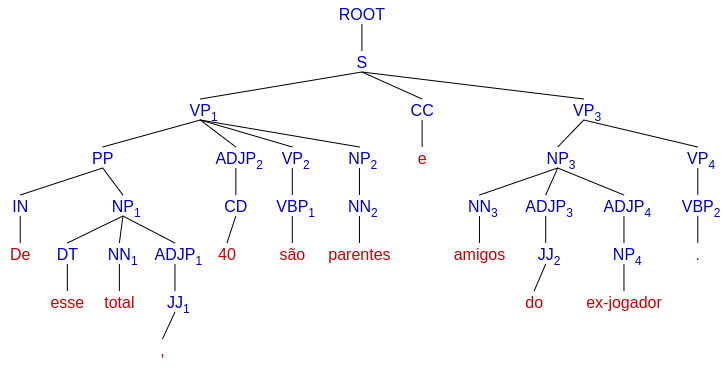
\includegraphics[width=\linewidth]{imagens/ec_bosque_ec_tree_ps.png}
        \caption{árvore gerada pelo SP}
    \end{minipage}
    \caption[Estudo de caso BOSQUE - Sentença transduzida com \textit{ec}, e \textit{cu}]{Estudo da sentença CF866-2, \textquote{De esse total, 40 são parentes e amigos do ex-jogador.}, que possui a \textit{tag} \textit{ec}. Em a), vemos a árvore relativa à sentença original no BOSQUE. Em b), a sentença pós transdução. E em c), a mesma sentença, classificada pelo SP com uma gramática gerada por este trabalho}
    \label{fig:ec_bosque_ec_tree}
\end{figure}